% !TEX encoding = UTF-8
% !TEX TS-program = pdflatex
% !TEX root = ../tesi.tex

%**************************************************************
\chapter{Analisi dei requisiti}
\label{cap:analisi-requisiti}
%*********************************************************

\section{Descrizione del prodotto}
\label{sec:descrizioneProdotto}
Il prodotto realizzato permette di effettuare interrogazioni all'interno del \gls{corpus}. Una volta che l'utente immette la ricerca (vedi fig. \ref{fig:esempioImplRicerca})
\begin{enumerate}
    \item si determinano i documenti pertinenti;
    \item i documenti recuperati vengono aggregati in base al loro ID;
    \item per ogni documento recuperato, si determina un punteggio di pertinenza;
    \item si visualizzano i risultati aggregati, ordinati in base al punteggio.
\end{enumerate}

Nella pagina di ricerca, una volta inserito cosa si sta cercando all'interno del form e premuto il tasto \texttt{Search}, viene recuperata una lista di documenti pertinenti all'interrogazione.

Esempio: assumiamo che i punteggi calcolati siano: 
\begin{center}
    \begin{tabular}{cc}
        \toprule
        ID documento & Punteggio \\
        \midrule
          2 & 105 \\
          27 & 100 \\
          19 & 88\\
          18 & 60\\
          23 & 42\\
          17 & 19\\
          4 & 16\\
          3 & 13\\
        \bottomrule
    \end{tabular}
        \captionof{table}[Esempio punteggi dei documenti pertinenti]{Esempio punteggi dei documenti pertinenti} 
        \label{tab:punteggiDocumentiPertinenti}
    \end{center}

il risultato aggregato sarà:

    \begin{center}
        \begin{tabular}{cc}
            \toprule
            ID documenti \\
            \midrule
            2, 3, 4 \\
            27\\
            17, 18, 19\\
            23\\
            \bottomrule
        \end{tabular}
            \captionof{table}[Risultato aggregato]{Risultato aggregato} 
            \label{tab:risultatoAggregato}
        \end{center}
Si noti che, sebbene il documento 3 abbia un punteggio inferiore al tutti gli altri i documenti pertinenti, è "premiato" dal fatto di essere aggregato al documento 2: la scelta di presentare così i risultati deriva dal fatto che i documenti del \gls{corpus} non sono unità separate (i.e. filmati diversi), ma dei frammenti audio.


%**************************************************************
\intro{Il capitolo descrive brevemente qual è il problema che bisognava affrontare, il prodotto realizzato ed elenca i requisiti individuati.}\\
\begin{figure}
    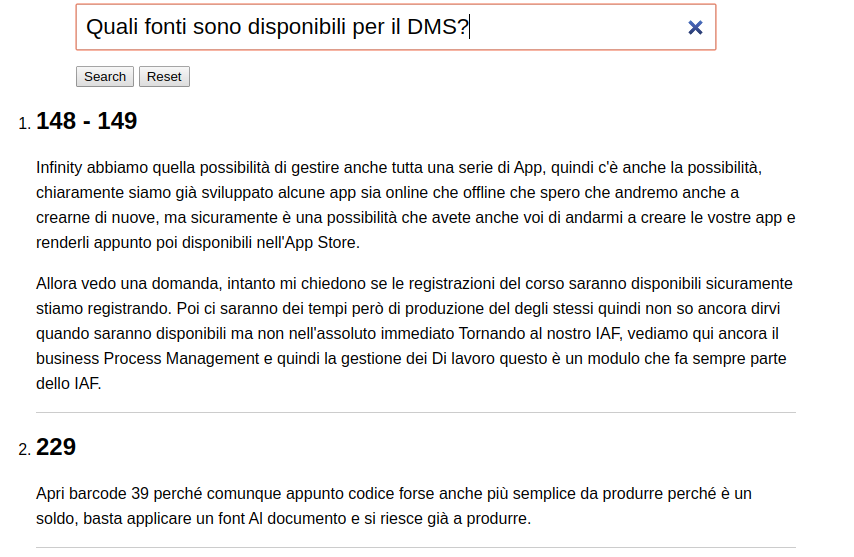
\includegraphics[scale=0.45]{immagini/ricerca.png}
    \caption{Esempio implementazione della ricerca}
    \label{fig:esempioImplRicerca}
 \end{figure}

\section{Migliorare la ricerca}
Quando si cerca di recuperare una informazione dal \gls{corpus} fornitomi dall'azienda, si presentano due problematiche principali:
\begin{itemize}
    \item il concetto che cerchiamo è presente nel testo trascritto, ma espresso in termini diversi (p.es. sinonimi, acronimi vs scritto per esteso);
    \item il concetto che cerchiamo non è presente nel testo trascritto, ma lo era nel filmato originale (i.e. errori di trascrizione). 
\end{itemize}

Capire se un concetto è presente o meno in un dato documento, avendo a disposizione solo la trascrizione, non è sempre evidente neanche per un classificatore umano: questo perché gli errori introdotti dal sistema di trascrizione rendono difficile, a volte impossibile, capire il senso delle frasi. Alcuni esempi degli errori di trascrizione presenti sono disponibili nel §\ref{cap:esempi-errori}.

%*********************************************************

\section{Requisiti}
Di seguito viene riportata una lista completa di tutti i requisiti individuati all'inizio dell'attività di stage. Ad ogni requisito viene assegnato il codice identificativo univoco:
\begin{center}
    \texttt{R[Tipo][Numero]}    
\end{center}
in cui ogni parte ha un significato preciso:
\begin{itemize}
    \item Numero: numero progressivo che segue una struttura gerarchica
    \item Tipo: la tipologia di requisito che può essere di:
    \begin{itemize}
        \item F: funzionalità.
        \item Q: qualità.
        \item V: vincolo.
    \end{itemize} 
\end{itemize}

Esempio: RQ2 indica il secondo requisito ed è un requisito di qualità.

\begin{longtable}{lp{.48\textwidth}p{.15\textwidth}}
    \toprule
        \thcell{Id Requisito} & \thcell{Descrizione} & \thcell{Fonte}\\
        \midrule
        \endfirsthead
        % intestazione normale
        \multicolumn{3}{l}{\footnotesize\itshape
        Continua dalla pagina precedente} \\
        \toprule
        \thcell{Id Requisito} & \thcell{Descrizione} & \thcell{Fonte}\\
        %\midrule
        \endhead
        % piede normale
        %\midrule
        \multicolumn{3}{r}{\footnotesize\itshape
        Continua nella prossima pagina} \\
        \endfoot
        % piede finale
    \bottomrule
    \caption[Requisiti individuati]{Requisiti individuati}
    %\multicolumn{3}{r}{\footnotesize\itshape Si conclude dalla pagina precedente} 
    \\
    \endlastfoot
        RF1 & L'utente deve poter effettuare una ricerca all'interno del \gls{corpus} & Azienda \\ \addlinespace
        RF2 & Implementazione di una collezione di test per valutare il sistema di ricerca mediante calcolo della precision, recall e f-measure& Azienda \\ \addlinespace
        RF3 & Implementazione di una pagina di ricerca dei documenti all'interno del \gls{corpus} che utilizzi un tesauro generato manualmente & Azienda\\ \addlinespace
        RF4 & Implementazione di una pagina di ricerca dei documenti all'interno del \gls{corpus} che utilizzi un \gls{autoencoder}\glsfirstoccur{} & Azienda\\ \addlinespace
        RF5 & Implementazione di una pagina di ricerca dei documenti all'interno del \gls{corpus} che utilizzi l'analisi della semantica latente & Azienda\\ \addlinespace
        RF6 & Implementazione di una pagina di ricerca dei documenti all'interno del \gls{corpus} che utilizzi un \gls{autoencoder} & Azienda\\ \addlinespace
        RF7 & Implementazione di una pagina di ricerca dei documenti all'interno del \gls{corpus} che utilizzi di un \gls{ensemble}\glsfirstoccur{} dei metodi (tesauro manuale, tesauro automatico, analisi della semantica latente e \gls{autoencoder}) & Azienda\\ \addlinespace
        RF8 & Implementazione di una pagina di ricerca dei documenti all'interno del \gls{corpus} che utilizzi un tesauro generico (di LibreOffice) & Azienda\\ \addlinespace
        RF9 & I risultati delle ricerche devono essere aggregati per ID continui, quindi ordinati in base allo score & Interno \\ \addlinespace
        RF10 & Configurazione dello stemmer italiano & Azienda \\ \addlinespace
        RV11 & Il prodotto deve essere eseguibile da browser (su Windows 10, browser Chrome $\geq$ 77.0.3865) & Interno \\ \addlinespace
        RQ12 & Deve essere fornita documentazione in inglese del codice in formato \gls{jsdoc} & Azienda/Interno \\ \addlinespace
%%%%%% end data
\label{tabella:requisitiIndividuati}
\end{longtable}

